
\documentclass[a4paper,11pt,twoside]{scrartcl}
\usepackage[utf8x]{inputenc}
\usepackage{graphicx}
\usepackage{geometry}
\usepackage[ngerman]{babel}
\usepackage{babelbib}
%\usepackage[backend=biber]{biblatex}
\usepackage{units}
\usepackage{url}
\usepackage{setspace}
\usepackage[
	pdftitle={Energie_Suffizienz},
 	pdfauthor={et.al.},
% 	pdfsubject={},
% 	pdfkeywords={},
	pdfstartview=FitH, % Auf Seitenbreite anpassen (Anzeige)
	pdfborder={0 0 0},
%  	bookmarks=true,
% %	plainpages=false,
	colorlinks=false,
	hyperfootnotes=false,
	pagebackref=false]{}
\usepackage[colorinlistoftodos,prependcaption,textsize=normalsize]{todonotes}  % disable
\usepackage{amsmath}
\usepackage{amstext}
\usepackage{amssymb}
\usepackage{color}
\usepackage[numbers]{natbib}
\usepackage{pdfpages}
\usepackage{hyphenat}
\usepackage{pdflscape} % für drucken ändern auf package lscape /pdflscape
\usepackage{textpos}
\usepackage{microtype}
\usepackage{enumitem}
\usepackage{multirow}
\usepackage{pdfcomment}

%\usepackage{hyperref}
%\hypersetup{
%    colorlinks=true,
%    linkcolor=gray,     
%    urlcolor=gray,
%}
%\usepackage{doi}

\usepackage{pgfgantt} % gantchart für den Arbeitsplan

% \usepackage{hyphenat}
\usepackage{float}
\usepackage{placeins}
\RequirePackage[bf]{caption}

\renewcommand{\textfraction}{.01} % vorher: .2
\renewcommand{\floatpagefraction}{.99}% vorher: .5
\renewcommand{\topfraction}{0.9}	% max fraction of floats at top
\renewcommand{\bottomfraction}{0.9}	% max fraction of floats at bottom

\newcommand{\ltab}{\raggedleft\arraybackslash}
\newcommand{\ctab}{\centering\arraybackslash} 
\newcommand{\rtab}{\raggedright\arraybackslash}

\usepackage{tabularx}
\newcolumntype{L}[1]{>{\raggedright\arraybackslash}p{#1}} % linksbündig mit Breitenangabe
\newcolumntype{C}[1]{>{\centering\arraybackslash}p{#1}} % zentriert mit Breitenangabe
\newcolumntype{R}[1]{>{\raggedleft\arraybackslash}p{#1}} % rechtsbündig mit Breitenangabe

\newcommand{\rem}[1]{}

% \renewcommand{\figurename}{Abb.}
% \renewcommand{\tablename}{Tab.}

\usepackage{acronym}
%\renewcommand{\bflabel}[1]{\normalfont{\normalsize{#1}}\hfill}

\usepackage[automark]{scrpage2}
\pagestyle{scrheadings}
\clearscrheadfoot
\ohead{\headmark}
\ofoot{\pagemark}
\setheadsepline{0.4pt}
\setfootsepline{0.4pt}

\setkomafont{pageheadfoot}{\rmfamily\small}

\renewcommand{\thefigure}{\arabic{section}-\arabic{figure}}
\renewcommand{\thetable}{\arabic{section}-\arabic{table}}

\newcommand{\entspricht}{\mathrel{\widehat{=}}}

\geometry{left=20mm,right=20mm, top=20mm, bottom=20mm}
\parindent 0pt
\parskip 11pt

% kein Platz zwischen \items
\setlist{nosep}
% Platz nach Überschriften reduzieren
\usepackage{titlesec}
\titlespacing*{\section}{0pt}{0pt}{0pt}
\titlespacing*{\subsection}{0pt}{0pt}{0pt}
\titlespacing*{\subsubsection}{0pt}{0pt}{0pt}
\titlespacing*{\paragraph}{0pt}{0pt}{5pt} % horizontal spacing in paragraph

\begin{document}
\onehalfspacing

\clearpage


{%\singlespacing

\thispagestyle{empty}
\begin{center}

%first row logos
\begin{figure}[htb]
    \centering
    \begin{minipage}[c]{0.3\linewidth}
        \centering
        
\includegraphics[width=4.5cm]{logos/europa-universitaet-flensburg-hauptlogo-rgb-600dpi.png}
    \end{minipage}
    \hfill
    \begin{minipage}[c]{0.35\linewidth}
        \centering
        \includegraphics[width=5cm]{logos/Logo_interdiszi_institut.png}
    \end{minipage}
    \hfill
    \begin{minipage}[c]{0.3\linewidth}
        \centering
        \includegraphics[width=2.5cm]{logos/Logo_wuppertal.png}
    \end{minipage}
\end{figure}

\iffalse
%second row logos
\begin{figure}[htb]
    \centering
    \begin{minipage}[c]{0.3\linewidth}
        \centering
        \includegraphics[width=2.2cm]{logos/2015_Logo_TUM_RGB.jpg}
    \end{minipage}
    \hfill
    \begin{minipage}[c]{0.35\linewidth}
        \centering
        \includegraphics[width=5.5cm]{logos/isea_rwth_logo.jpg}
    \end{minipage}
    \hfill
    \begin{minipage}[c]{0.3\linewidth}
        \centering
        \includegraphics[width=3cm]{logos/TU_Logo_lang_RGB_rot.png}
    \end{minipage}
\end{figure}
\fi
\vspace*{1 cm}

{\LARGE\textbf{\textsf{Skizze Nachwuchsforschungsgruppe}}

\textsf{\textit{im Rahmen der Bekanntmachung \glqq inter- und transdisziplinär arbeitende Nachwuchsgruppen im Rahmen der Sozial-ökologischen Forschung\grqq} }
}

\vspace{0.5cm}

{\Huge
\textbf{\textsf{Die Rolle von Energie-Suffizienz in Energiewende und Gesellschaft}}

\textbf{\textsf{}}
}

{\Huge
\textbf{\textsf{Akronym:{EnSufGe}}}
}

\vspace{1cm}

Eingereicht durch
Frauke Wiese\\
i$^{2}$ Interdisziplinäres Institut für Umwelt-, Human- und Sozialwissenschaften\\
Europa-Universität Flensburg, Auf dem Campus 1, 24943 Flensburg


\vspace{0.5cm}

An den Projektträger im DLR \\
AE 41 Globaler Wandel/Klima- und Umweltschutz, Sozial-ökologische Forschung \\
Heinrich-Konen-Straße 1, 53227 Bonn


\end{center}
\iffalse
\begin{table*}[b]
\centering
\footnotesize
\begin{tabular}{ | p{5cm} | p{5cm} |} \hline
\textbf{Konsortialpartner} & \textbf{Modelle/Frameworks} \\ \hline
Reiner Lemoine Institut & Leitung des Experiments \\ \hline
Technische Universität München & urbs \\ \hline
Europa-Universität Flensburg & oemof \\ \hline
RWTH Aachen & GENESYS-2 \\ \hline
Technische Universität Berlin & OSeMOSYS \\ \hline
Dänische Technische Universität & Balmorel \\ \hline
\end{tabular}
\label{tab:Partner}
\end{table*}
\fi


\clearpage
}

\setcounter{page}{1}

\section{Zielstellung und gesellschaftlicher Bedarf}
\label{sec:ziel}
%\textit{Beschreibung der Problem- und Zielstellung sowie des gesellschaftlichen Bedarfs}
Energiesystem-Modelle sind etablierte Werkzeuge, um technisch mögliche und ökonomisch vorteilhafte Energiewende-Pfade im Zusammenspiel von Effizienz- und Konsistenz-Strategien abzubilden. Sie sind inzwischen zu einer Grundlage politischer Entscheidungen und Steuerung sowie Gegenstand wissenschaftlicher Debatten geworden. Allein: Gesellschaftliche Entwicklungen, die eine Reduktion des absoluten Energieverbrauchs durch veränderte Praktiken und Routinen im Sinne einer Suffizienz-Strategie ermöglichen, werden bisher kaum berücksichtigt \cite{SAMADI2017}. Die Nachfrage-Seite wird in bestehenden Modellen in der Regel über technologische Änderungen (Effizienzmaßnahmen) abgebildet. Die Nachfrage selbst wird kaum hinterfragt \cite{Creutzig2018} und die hinter den Eckdaten liegenden Annahmen werden nicht explizit gemacht.

\begin{table}[h]
\begin{center}
\small
  \caption{Bedeutung der Begriffe in Bezug auf Energiewende}
\begin{tabular}[h]{|l | l |}
\hline
&\\
Konsistenz & Erneuerbare Energien ersetzen Fossile\\
&\\
\hline
&\\
 Effizienz & Relative Reduktion des Energieverbrauchs bei Bereitstellung der gleichen\\
 & Energiedienstleistung\\
 \hline
 &\\
Suffizienz & Absolute Reduktion des Energieverbrauchs durch soziale Innovationen, Exnovationen\\
& und verändertes Nutzungsverhalten \\
 \hline
 \end{tabular}
 \label{tab:koefsu}
\end{center}
\end{table}

Bislang sind Modellierungen weitgehend blind gegenüber Veränderungen durch gesellschaftlichen Wandel und berücksichtigen hier liegende Potenziale und Risiken nicht. Zudem kommen eng mit der Energiewende verknüpfte Aspekte wie Ressourcenbedarf \cite{Mocker2015,Buchert2011} Akzeptanzfragen \cite{Fuchs2016}, Flächenverbrauch \cite{Rink2011}, planetare Belastungsgrenzen \cite{Rockstroem2009} oder den Sustainable Development Goals \cite{UN_SDG} wenig vor. \\
Hier setzt die Nachwuchsgruppe an: In Anlehnung an Albert Einstein liegt der Ausgangspunkt des Forschungsvorhabens darin, dass Probleme nicht mit derselben Rationalität gelöst werden können, die sie hervorgebracht haben. Zwar ist die zentrale Herausforderung einer Energiewende in Deutschland angesichts von Klimawandel, Ressourcenverknappung und Risikotechnologien erkannt, doch die Debatten und vorgeschlagenen Maßnahmen verbleiben überwiegend in alten Rationalitätsmustern: Die Energiewende wird unter den Aspekten von Kosten, Marktpotenzialen und technischer Machbarkeit (Effizienz und Konsistenz) verhandelt, während Treiber vermehrten Energieverbrauchs – wie das modernen Gesellschaften inhärente Wachstumsparadigma oder zunehmende Innovationsgeschwindigkeit – kaum problematisiert werden.\\
Vor diesem Hintergrund liegt das übergreifende Ziel des angestrebten Nachwuchsverbundes darin, Suffizienzaspekte und -strategien für die Energiesystem-Modellierung zu operationalisieren und damit handlungsbasierte Parameter und gesellschaftlichen Wandel in Energie- und Klimaschutzszenarien darstellen zu können. Die Parameter werden dabei mit Instrumenten, Handlungsoptionen und veränderten Rahmenbedingungen explizit hinterlegt. Hierfür gilt es, gesellschaftliche Transformationsprozesse im Kontext der Energiewende besser zu verstehen, die Blockaden für und Potenziale von Suffizienzpolitiken auszuloten und nicht zuletzt im Sinne einer globalen Nachhaltigkeit mögliche Externalisierungs- und Verlagerungseffekte zu diskutieren. 

\section{Stand von Wissenschaft und Technik sowie eigene Vorarbeiten}
\label{sec:2}
Nachhaltigkeitsforschung, sozial-ökologische Forschung und Transformationsforschung sind seit langem mit Fragen der Umsetzung befasst: Wie ist es möglich, vom Wissen zum Handeln zu kommen? \cite{BMBF2008} Wie kann geschehen, was geschehen muss? \cite{Linz2000} Und wie können Klimaschutzziele, wie kann ein deutlich geringerer Naturverbrauch erreicht werden, ohne zivilisatorische Errungenschaften zu gefährden? \cite{Sommer2016,WGBU2011} Die Antworten fallen unterschiedlich aus und die Bearbeitung dieser Frage geschieht in unterschiedlicher Weise.

\subsection*{Energiesystem-Analyse und Modellierung}
Energiesystem-Modelle sind Werkzeuge um Orientierungswissen zu Energiewendepfaden zu generieren. So wurden mit ihrer Hilfe die Realisierbarkeit von 100\% Erneuerbare Energien Strom-Systemen dargelegt, sowohl für Deutschland \cite{SRU2011} als auch für Europa \cite{Hohmeyer2015}. Inzwischen geht es in der ökonomisch-technisch geprägten Energiesystem-Analyse nicht mehr um das \textit{ob}, sondern eher um das \textit{wie} der Energiewende und  eine steigende Anzahl komplexer Modelle wird genutzt, um Chancen der Sektorkopplung von Strom, Wärme, Mobilität \cite{Quaschning2016} einzuschätzen, Marktregeln bei hohem Anteil Erneuerbarer Energien zu erörtern, sowie Netz- \cite{openEgo2015} und Speicherbedarf \cite{ANGUS2017} abzuschätzen. \\
Zu Richtungsentscheidungen für Energiewendepfade nehmen Energiesystem-Modelle somit eine wichtige Rolle in Wissenschaft und politischer Beratung zu Klima- und Energiepolitik ein \cite{Dieckhoff2015}. In den letzten Jahren werden die Modelle jedoch für ihren Black-Box-Charakter kritisiert \cite{Pfenninger2017, Pfenninger2017b,Cao2016}. Wiese \citep{Wiese2015} zufolge besteht ein hoher Bedarf an Transparenz in der Energiesystem-Modellierung, um eine partizipative Energiewende zu ermöglichen \cite{Wiese2014}. Auch wird ein Bedarf an interdisziplinären Ansätzen in der Energiesystem-Modellierung identifiziert \cite{Wiese2018,Pfenninger2014,Schuitema2017}. Die  Sozialwissenschaften sind für eine gesellschaftliche Energiewende von großer Bedeutung \cite{Sovacool2015}, jedoch völlig unterrepräsentiert in der Energiesystemforschung \cite{Sovacool2014}.\\
Die Energiesystem-Analyse an der EUF trägt mit der Bereitstellung von offenen Modellen \cite{renpass,renpassGIS} und einem Modellierungs-Framework \cite{oemof} zu der nötigen Transparenz der Energiesystem-Analyse bei. Im Projekt "verNetzen" \cite{vernetzen2016} wurde die Verknüpfung von sozialwissenschatlichen Ansätzen mit der Energiewende-Modellierung in Bezug auf Akzeptanz von Windkraftanlagen und Netzausbau erprobt. Die Energiemodellierung als Werkzeug wird im Hinblick auf ihre Nützlichkeit von den Modellierer*innen selbst beständig hinterfragt \cite{Wiese2018}.

\subsection*{Sozial-ökologische Transformationsforschung}
Die Energiesystem-Modellierung stellt immer wieder dar, dass die Etablierung einer klimafreundlichen und nachhaltigen Energieversorgung grundsätzlich technisch machbar und ökonomisch zu bewältigen wäre. Für die Trägheit mit der dies geschieht, werden vor allem gesellschaftliche Barrieren und Zwänge ausgemacht.
Entsprechend werden in der sozial-ökologischen Transformationsforschung Transformationshemmnisse auf der Mikro-, Makro und Mesoebene gesellschaftlicher (Re-)Produktion identifiziert und analysiert, nachhaltige Praktiken und die Bedingungen ihrer Diffusion erforscht \cite{Kny2015} oder untersucht, wie Nachhaltigkeit im Feld der Wirtschaft von verschiedenen Instrumenten unternehmerischer Verantwortung adressiert und eingefordert wird \cite{Sommer2016b}. 
Sozial-ökologische Krisen lenken den Blick auf die künftige energetische Basis moderner Gesellschaften. In diesem Kontext wird seit längerer Zeit der Stellenwert der Suffizienz thematisiert \cite{Huber1995,Fischer2013,Schneidewind2013}. Zielt die Suffizienzstrategie doch auf die Senkung des absoluten Ressourcenverbrauchs, mithin auch auf eine grundlegende Transformation gesellschaftlicher Werte und Normen und mentaler Infrastrukturen.\\
Die Rekonstruktion umfassenden gesellschaftlichen Wandels in der Vergangenheit dient in der Transformationsforschung, wie sie am Norbert Elias Center (NEC) betrieben wird, einerseits dem besseren Verständnis des Gewordenseins gegenwärtiger Verhältnisse. Andererseits können aus den gewonnenen Erkenntnissen Handlungsoptionen, mögliche Entwicklungslinien und Gestaltungsszenarien für zeitgenössische und künftige sozial-ökologische Wandlungsprozesse abgeleitet werden \cite{Christ2015,Christ2016}. Gegenwartsorientierte Forschungsarbeiten zielen darauf ab, soziale, politische und ökonomische Ursachen und Folgen von sozial-ökologischen Krisen, wie etwa dem Klimawandel, zu identifizieren \cite{Sommer2011,Sommer2015,Stumpf2015}.\\ 
Die energetische Basis historischer und moderner Gesellschaften spielt dabei eine zentrale Rolle. Bezogen auf die Transformation des Energieregimes kann konstatiert werden, dass Suffizienz im gesellschaftlichen Diskurs bislang noch von geringer Relevanz ist – obwohl die Reflektion der ergriffenen Maßnahmen zeigt, dass diese zur Senkung des absoluten Verbrauchs nicht ausreichen werden \cite{Brischke2016}. Welche gesellschaftlichen Beharrungskräfte die Verbreitung von Suffizienz verhindern und welche Handlungsspielräume es für diese Strategie in urbanen Räumen gibt, steht gegenwärtig im Fokus des BMBF geförderten und am NEC bearbeiteten Forschungsprojekts „Entwicklungschancen und -hemmnisse einer suffizienzorientierten Stadtentwicklung (EHSS)“ (2017-2020). 
\subsection*{Sufizienzpolitik}
Anders als Effizienz und Konsistenz ist Suffizienz mit einem grundlegenden Strukturwandel verbunden, der nicht ausschließlich technologische sondern vor allem gesellschaftliche Dimensionen umfasst. Oft wird er mit der moralischen Ebene (Verzicht) assoziiert, mit Konsumverhalten verknüpft und so auf eine Verantwortung des Individuums reduziert. Als Nachhaltigkeits-Strategie mit einer politischen Dimension ist Suffizienz lange kaum debattiert worden \cite{Winterfeld2002}. Erst im Kontext der sich ab 2010 neu entzündenden wachstumskritischen Debatte wurde der Begriff vermehrt aufgegriffen und bearbeitet \cite{Seidl2010,Raetz2011,Schneidewind2013,Winterfeld2017,Linz2015,Bierwirth2015,Thomas2015,Adler2017}. Die internationale Debatte zu Suffizienzpolitiken wird stark durch den ökofeministischen Ansatz von \cite{Salleh2009} mit geprägt und ergänzt aus der Perspektive des globalen Südens den Ansatz des „Savings“ (das Recht, etwas übrig zu behalten im Kontext der Armutsbekämpfung).\\
Die Forschung und Arbeit zu Suffizienzpolitik ist am Wuppertal Institut seit vielen Jahren verankert (vgl. Verweise auf Wolfgang Sachs, Manfred Linz, Uwe Schneidewind u.a.).
Neben den genannten Publikationen umfassten die Arbeiten zu diesem Thema in den letzten Jahren insbesondere das Projekt „Energiesuffizienz“ \cite{Brischke2016} im Rahmen der Sozial-ökologischen Forschung des BMBF sowie das Projekt „Policy Guide: Energy Sufficiency in Buildings“ \cite{EnergySufficiencyProjekt} zur Entwicklung suffizienzpolitischer Maßnahmen für die europäische Ebene. Darüber hinaus bestehen umfangreiche Erfahrungen in der Bearbeitung inter- und transdisziplinärer Projekte, der interdisziplinären Modellierung sowie in der methodischen Entwicklung zur Integration sozialwissenschaftlicher Empirie in die Modellierung \cite{Bierwirth2016}.

Während die Integration von Suffizienzpolitiken und Transformationserzählungen in Ansätzen schon erfolgt, stellt die suffizienzbasierte Modellierung eine noch kaum abschätzbare Herausforderung dar \cite{SAMADI2017}. Eine gelungene inter- und transdisziplinäre Verkopplung aller drei Teilbereiche bedarf neuer Theorieansätze (z.B. zur „Externalisierung“) wie neuer methodologischer und methodischer Ansätze einschließlich quantitativ-qualitativer Verkopplungen.

\section{Bezug zur Sozial-ökologischen Forschung und zu den Förderzielen}
Erster Bezugspunkt zur Sozial-ökologischen Forschung ist die Interdisziplinarität des beabsichtigten Nachwuchsforschungsverbundes über die Zusammenarbeit von Technik- und Sozialwissenschaftler*innen. Mit der Weiterenwicklung interdisziplinärer Szenario-Methoden und deren Anwendung trägt die Nachwuchsforschungsgruppe zur Integration disziplinären Wissens für Energiewende und Klimaschutz bei.\\
Zweiter Bezugspunkt ist der transdisziplinäre Ansatz. Im Projekt ist eine enge Zusammenarbeit mit kommunalen Praxispartner*innen bei der Szenarienerstellung und -bewertung vorgesehen, wobei auf bestehende Kooperationen aufgebaut werden kann.\\
Weiter und in Bezug zu den Förderzielen soll sowohl die internationale Dimension (z.B. Auswirkungen deutscher Energiewendepolitiken auf andere Länder) als auch der über die Integration der Genderdimension mögliche Perspektivwechsel in den Promotionsvorhaben bearbeitet werden. Thematisch widmet sich die Nachwuchsforschungsgruppe einer in der Sozial-ökologischen Forschung als zentral geltenden Nachhaltigkeits-Herausforderung: Der umwelt- und gesellschaftsverträglichen Transformation des Energiesystems. Mit der Fokussierung auf Suffizienz nehmen die Nachwuchswissenschaftler*innen Bezug zu Ressourcenschonung sowie dem Sozial-ökologischen Forschungs-Schwerpunkt Nachhaltiges Wirtschaften.\\
Die Weiterentwicklung institutioneller Kapazitäten zur Durchführung transdisziplinärer Nachhaltigkeitsforschung wird durch die Verankerung der Nachwuchsgruppe am Interdisziplinären Institut für Umwelt-, Sozial und Humanwissenschaften an der Europa-Universität Flensburg (EUF) sowie am Wuppertal Institut (WI) geschaffen. Der Wissensaustausch zwischen Universität und außeruniversitärer Forschungseinrichtung wird durch die gemeinsame Leitung intensiviert. In der eigenverantwortlichen Arbeitsgruppe bekommen junge Wissenschaftler*innen die Möglichkeit sich weiter zu qualifizieren, sich auf der Basis ihres disziplinären Vorwissens Sozial-ökologischen Fragestellungen zu widmen und gemeinsam Transformationswissen hervorzubringen \cite{Schneidewind2014}.

\section{Forschungsarbeit und Arbeitsprogramm}
\label{sec:4}
%\textit{Beschreibung der geplanten Forschungsarbeiten und des Arbeitsprogramms, unter Einschluss der Darstellung von Methoden, die zur Anwendung kommen bzw. entwickelt werden sollen; sowie der disziplinären Zusammensetzung der geplanten Nachwuchsgruppe}
\begin{figure}[!h]
    \centering
    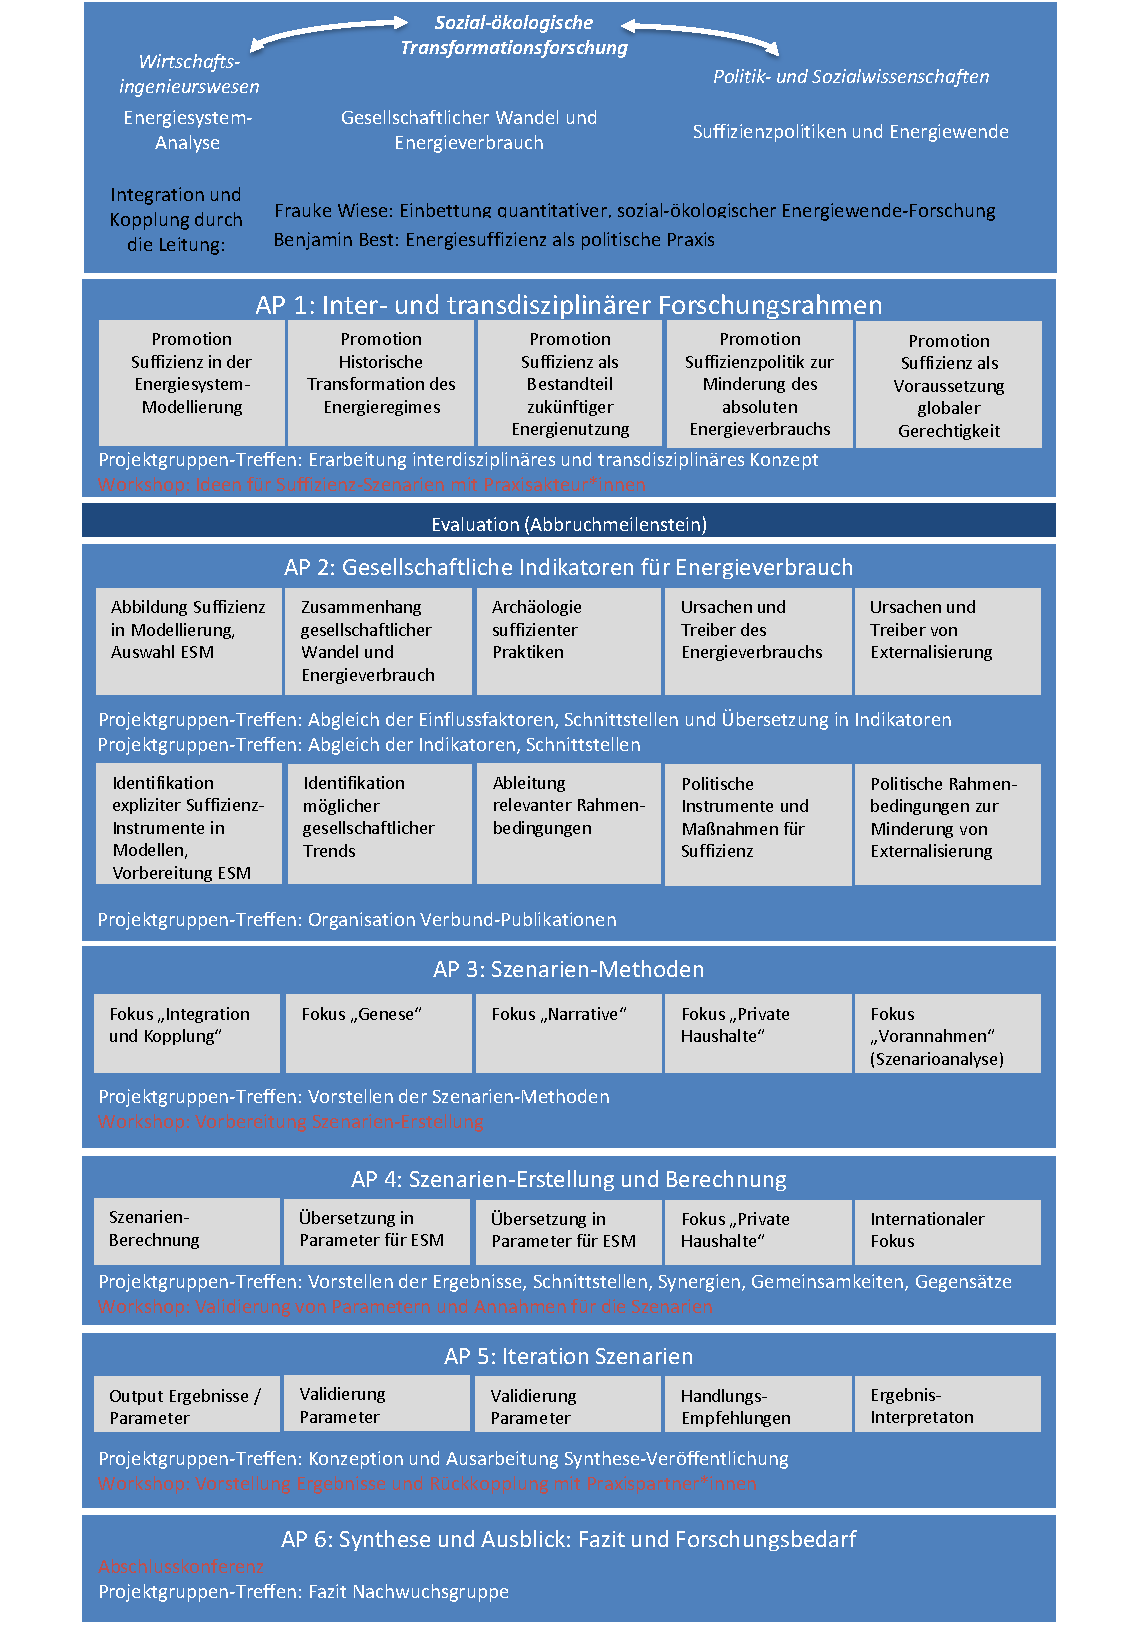
\includegraphics[width=0.9\textwidth]{figures/Forschungsarbeit4+Uta_2_Frauke3.pdf}
    \caption{Forschungsprogramm der Nachwuchsforschungsgruppe}
    \label{fig:forschungsprogramm}
\end{figure}

Das Nachwuchsforschungsvorhaben enthält drei Forschungsschwerpunkte, in denen fünf Promotionsvorhaben angesiedelt sind (in Abbildung \ref{fig:forschungsprogramm} vertikal dargestellt), die über sechs interdisziplinäre Arbeitspakete (horizontal dargestellt) ineinander greifen. 

\subsection{Forschungsschwerpunkte und Disziplinen}
Im Forschungsschwerpunkt \textit{Energiesystem-Analyse} soll sich unter der Leitung von Frauke Wiese ein*e Doktorand*in aus dem Bereich Wirtschaftsingenieurwesen auf die Abbildung von Suffizienz in Energiesystem-Modellen fokussieren. Das Promotionsvorhaben umfasst methodisch sowohl die Abbildung von Indikatoren aus dem sozialwissenschaftlichen Bereich in einem quantitativen Modell als auch die Berechnung von Energie-Szenarien, die Suffizienz neben Effizienz- und Konsistenz-Optionen abbilden. Die Modellierung soll auf einem bestehenden offenen Modell aufbauen und dieses um den Aspekt Suffizienz erweitern. Ob hierfür das u.a an der EUF erarbeitete Energiesystem-Modellierungs-Framework 'oemof' in der Nachwuchsgruppe genutzt und erweitert wird, bleibt einer genauen Prüfung und dem Vergleich mit anderen Optionen vorbehalten.

Im Forschungsschwerpunkt \textit{gesellschaftlicher Wandel und Energieverbrauch} der sozial-ökologischen Transformationsforschung (angesiedelt am NEC) sind zwei Promotionen vorgesehen: Eine wird in historischer Perspektive Zusammenhänge zwischen Energieverbrauch und sozialem Wandel herausarbeiten, mithin untersuchen, welche politischen, sozialen, soziokulturellen oder ökonomischen Dynamiken den Status quo des Energieverbrauchs hervorgebracht haben, um mögliche Ansatzpunkte für Transformationen sichtbar zu machen. Die zweite Arbeit ist dem Blick in wahrscheinliche, mögliche und wünschbare Zukünfte \cite{Kreibich2008} und der Frage gewidmet, wie gesellschaftliche Veränderungen und Trends künftig mit Energieverfügbarkeit und -nachfrage interagieren werden. Aus beiden zeitlichen Perspektiven – der historischen Rekonstruktion wie dem Blick auf vermutbare Zukünfte – werden sich Möglichkeiten und Grenzen (etwa aufgrund von Pfadabhängigkeiten, nicht intendierten Nebenfolgen, Rebound-Effekten etc.) für einen suffizienten Umgang mit Energie bzw. eine absolute Reduktion des Energieverbrauchs ableiten lassen.

Der Forschungsschwerpunkt \textit{Suffizienzpolitiken und Energiewende} ist am Wuppertal Institut verortet und wird von Benjamin Best geleitet. Hierin sollen zwei Promotionen mit sozial- bzw. politikwissenschaftlichem Hintergrund entstehen. Eine Dissertation beschäftigt sich mit der Gestaltung von politischen Rahmenbedingungen und ihren Wechselwirkungen mit energierelevanten sozialen Praktiken, Verhaltensweisen und Routinen. Die übergeordnete Fragestellung wird sein, inwiefern Politik und veränderte Rahmenbedingungen suffizientes Verhalten befördern, behindern oder allgemein beeinflussen können. Das zweite Promotionsvorhaben ist in der Politikwissenschaft und dem Ansatz der Politischen Ökologie angesiedelt. Ausgangspunkte sind „Imperiale Lebensweisen“ \cite{Brand2017}, Externalisierung \cite{Lessenich2016,BieseckerOJ} und die Frage nach globaler Gerechtigkeit (einschließlich der Geschlechtergerechtigkeit). Es soll untersuchen, inwiefern Suffizienzpolitiken zur Veränderung imperialer und externalisierender Grundkonstellationen beitragen können.

Der Fokus der Forschungsgruppenleiter*innen liegt auf der Integration und Kopplung der Forschungsarbeiten. Dabei konzentriert sich Frauke Wiese auf die stringente Einbettung quantitativer sozial-ökologischer Energiewende-Forschung in die Modellierung. Ziel ist es durch die interdisziplinäre Kooperation die „blinden Flecken“ der Energiesystem-Modellierung zu identifizieren und diese so weit wie möglich auszugleichen. Ein Zugang ist dabei die Integration der erarbeiteten Szenarien (Schwerpunkt Suffizienz) sowie die Ergebnisinterpretation und -verwendung. Getragen wird dies einerseits von der Frage an welcher Stelle und in welcher Form Modelle zu Erkenntnisgewinnen bzgl. Suffzienz in Energiewendepfaden beitragen können und wie andererseits Wissensbestände zur Suffizienz in Modellierungen abgebildet werden können. Im Schwerpunkt "Energiesuffizienz als politische Praxis" bewertet Benjamin Best die Forschungsergebnisse hinsichtlich ihrer Bedeutung für Suffizienzpolitiken und entwickelt daraus Instrumente für unterschiedliche Sektoren. Darüber hinaus liegt das Augenmerk von Benjamin Best auf dem Partizipationsprozess zur Anwendung der Szenario-Methodik, als ein Beispiel für eine transdisziplinäre Energieforschung. 


\subsection{Arbeitspakete und Methoden}
%Die Erkenntnisse aus den Arbeitspaketen werden von den Forschungsgruppenleiter*innen einerseits in das entstehende Energiesystemmodell integriert und andererseits zur kritischen Reflexion bestehender energiepolitischer Steuerungsinstrumente genutzt.
\subsubsection*{AP1: Inter- und transdisziplinärer Forschungsrahmen}
In AP1 wird von allen Gruppenmitgliedern der interdisziplinäre Bezugsrahmen entworfen und das transdisziplinäre Forschungsdesign gemeinsam konkretisiert. Im Rahmen eines Auftakt-Workshops mit den Promovierenden werden die bis dahin zu erstellenden Kurz-Expoés zu Promotionsideen vorgestellt und diskutiert.
In diesem Zusammenhang wird ausgelotet, inwiefern eine inhaltliche, thematische oder sektorale Fokussierung in einzelnen Promotionen sinnvoll oder notwendig ist (z.B. Privathaushalte, Mobilität, spezifische Zielgruppen, geografische Verortung) und welche Praxis-Akteur*innen einbezogen und beteiligt werden sollen. Im Rahmen eines zweiten Workshops werden gemeinsam mit ausgewählten Akteur*innen Ideen für Suffizienzszenarien generiert.
Die Ergebnisse beider Workshops bilden die konzeptionelle Grundlage für die inter- und transdisziplinäre Zusammenarbeit und die gemeinsame Arbeit an Szenarien. Die Produkte P1-(1-3) des ersten Jahres sind die Ergebnisse für das Erreichen des ersten Meilensteins M1, die dem Projektträger zur Evaluation vorgelegt werden.
\begin{itemize}
    \item[\textbf{P1-1}] fünf Kurz-Exposés zu den Qualifikationsvorhaben 
    \item[\textbf{P1-2}] Konzept zur inter- und transdisziplinären Zusammenarbeit
    \item[\textbf{P1-3}] Konzept für die gemeinsame Arbeit an Szenarien 
    \item[\textbf{M1 :}] \textbf{Qualifikationskonzept sowie inter- und transdisziplinäres Forschungsdesign}
\end{itemize}

\subsubsection*{AP2: Gesellschaftliche Indikatoren für Energieverbrauch}
Um Suffizienz im Energiesystem-Model abbilden zu können, bedarf es einer Übersetzung von gesellschaftlichen Indikatoren zu quantifizierbarem Energieverbrauch. Dieser soziologisch-technisch-ökonomischen Schnittstelle ist AP2 gewidmet. Ziel ist es, relevante Faktoren und Parameter zu identifizieren, mit denen gesellschaftliche Dynamiken, die sich auf Energienachfrage und -verbrauch auswirken, abgebildet und in Datenform ausgedrückt werden können. Dazu wird, zunächst aus unterschiedlichen disziplinären Perspektiven und sowohl historisch als auch gegenwartsbezogen, nachgezeichnet, wie sich mit der Etablierung des fossilistisch und atomar basierten Energieregimes in der Vergangenheit sowohl Alltagspraktiken in den Bereichen Wärme, Mobilität, Strom (mit einer noch festzulegenden Schwerpunktsetzung, vgl. AP1) verändert haben als auch gesellschaftliche Reproduktionsweisen transformiert wurden. Gefragt wird, welche Implikationen dies jeweils für den Energieverbrauch bis heute hat, welche Zielgruppen und Sektoren besondere Beachtung finden sollen oder auch, welche Externalisierungsprozesse in die Analyse einbezogen werden müssen. Um Annahmen und Parameter um den Aspekt der Suffizienz zu erweitern bzw. in den Modellen abzubilden und explizit zu machen, müssen sie mit Instrumenten oder konkreten (politischen) Maßnahmen hinterlegt sein. Dementsprechend gilt es in diesem Schritt, einerseits bestehende Suffizienz-Politiken wie auch kontraproduktive Instrumente zu identifizieren und mögliche geänderte und neue Politiken und Rahmenbedingungen zu entwerfen. Diese Ansätze bilden die Grundlage für die Auswahl der Indikatoren, die in ein Energiesystem-Modell als Input-Parameter aufgenommen werden können, um Suffizienz explizit abzubilden. Die Synthese der jeweiligen Ergebnisse aus den fünf Promotionen findet entsprechend des in AP1 entwickelten Konzepts statt. 

\begin{itemize}
    \item[\textbf{P2-1}] Verbundpaper zu Treibern, Indikatoren, Auswirkungen und Perspektiven des Energieverbrauchs 
    \item[\textbf{P2-2}] Gemeinsames Forschungsteilprojektpaper zu Energie-Suffizienz-Politiken 
    \item[\textbf{M2 :}] \textbf{Theoretischer und konzeptioneller Rahmen der Qualifikationsvorhaben mit Bezug auf Blockaden und Chancen für Energie-Suffizienz-Politiken}
\end{itemize}

\subsubsection*{AP3: Szenarien-Methoden}
In diesem methodischen Arbeitspaket wird ein Verfahren für die Erstellung von konsistenten, multiperspektivischen Energieszenarien entwickelt. Hierfür ermittelt jede*r der fünf Promovend*innen Vorschläge für mögliche Szenario-Methoden, die geeignet sind, Energie-Szenarien im Zusammenhang mit gesellschaftlichen Entwicklungen zu erstellen.
Es können qualitative, erzählerische Szenarien eingesetzt werden, die im Sinne einer Meta-Studie auf der Auswertung relevanter Literatur zu spezifischen Themen beruhen. Es können sich aber auch quantitative Szenarien anbieten, wie sie in der Modellierung bereits eingesetzt werden, um durch die Variierung der Annahmen mögliche gesellschaftliche Trends und veränderte Rahmenbedingungen zu simulieren \cite{Bierwirth2016}. Neben „klassischen“ Forecasting-Szenarien \cite{Kosow2008} können Backcasting-Szenarien \cite{Robinson2003,Robinson2011} von einer normativen Vision für eine wünschbare Zukunft ausgehen – etwa einer lebenswerten Gesellschaft, die ohne (auch externalisierte) Emissionen im Energiebereich auskommt („Null Emissionen bis 2050“) – und methodisch kontrolliert abschätzen, welche notwendigen Schritte auf dem Weg in diese wünschenswerte Zukunft gegangen sein und welche Verhaltens- und gesellschaftlichen Veränderungen bis zum Zieljahr vollzogen worden sein müssten. Des Weiteren sind Ansätze relevant, die qualitative und quantitative Elemente der Systemanalyse verbinden \cite{WEIMERJEHLE2016}.\\
Im disziplinären Austausch wird geprüft, welche Methoden geeignet sind, um sozio-technische Transformationsszenarien im Hinblick auf Energie-Suffizienz zu erstellen. Im Rahmen der transdisziplinären Zusammenarbeit ist ein Zukunftsworkshop vorgesehen, der entsprechend der Methode der Szenario-Technik die Erstellung von Szenarien vorbereitet (siehe AP4).
\begin{itemize}
    \item[\textbf{P3-1}] Szenariokonzept 
    \item[\textbf{P3-2}] Verbundpaper zu Energieszenario-Methoden 
    \item[\textbf{M3 :}] \textbf{Entwicklung und Erprobung von Szenario-Ansätzen zu Energiesuffizienz}
\end{itemize}

\subsubsection*{AP4:Szenarien-Erstellung und Berechnung}
Im Anschluss an die Auswahl der Methoden kommen diese in AP4 zur Anwendung. In der inter- und transdisziplinären Arbeitsphase werden Energiesystem-Szenarien einmal mit Fokus auf Deutschland, einmal mit kommunalem Fokus und einmal mit einer internationaler Perspektive hinsichtlich zu vermeidender Externalisierung erstellt. Dabei werden nach Möglichkeit im Rahmen von Workshops und Befragungen die Praxispartner*innen in die Erstellung der sozio-technischen Szenarien einbezogen. Aus den Szenarien werden die Annahmen abgeleitet, die in die Energiesystem-Modellierung einfließen. Ein wichtiger Aspekt ist hierbei, dass implizite Annahmen über gesellschaftliche Entwicklungen, die in jedem Energie-Szenario enthalten sind, klar formuliert und explizit gemacht sowie mit konkreten Trends, Instrumenten oder veränderten Rahmenbedingungen hinterlegt werden. Außerdem werden in dieser Phase erste Berechnungen der erstellten Szenarien durchgeführt.

\begin{itemize}
    \item[\textbf{P4-1}] Dokumentation Workshop Szenario-Erstellung
    \item[\textbf{P4-2}] Veröffentlichung Programm-Code Energiesystem-Modell inkl. Suffizienz (Beta-Version)
    \item[\textbf{P4-3}] Verbundpaper zur Übersetzung qualitativer Daten in quantitative Eingangs-Parameter für Energiesystem-Modelle
    \item[\textbf{M4 :}] \textbf{Erste Version interdisziplinärer Energie-Szenarien inkl. Suffizienz liegt vor}
\end{itemize}

\subsubsection*{AP5:Iteration Szenarien}
Erfahrungsgemäß wird nach der konkreten Übersetzung der Szenarien in quantifizierte Daten und deren Einspeisung in ein Energiesystem-Modell deutlich, welche Eingangs-Parameter besonders großen Einfluss auf die Ergebnisse haben. Manche Parameter mögen einen größeren Einfluss haben als angenommen, andere haben vielleicht keinerlei Einfluss auf die Konfiguration des Systems und eventuell treten sogar Parameter zu Tage, die weitere implizite Annahmen über die gesellschaftliche Entwicklung beinhalten. Deshalb werden die Ergebnisse zuerst im Rahmen der regelmäßigen Treffen in der Projektgruppe interdisziplinär verifiziert und validiert, um im Anschluss die Szenarien in mindestens einer Iterations-Schleife anzupassen und zu erweitern. Hinsichtlich der transdisziplinären Einbindung der Praxis-Partner*innen, bietet sich an dieser Stelle eine weitere Veranstaltung an, die zentrale Parameter und die Ergebnisse der Modellierung präsentiert und zur Diskussion stellt.
\begin{itemize}
    \item[\textbf{P5-1}] Dokumentation des Workshops zur Rückkopplung der Ergebnisse mit Praxispartner*innen
    \item[\textbf{P5-2}] Handlungsempfehlungen Energie-Suffizienz
    \item[\textbf{P5-3}] Verbundpaper zur Abbildung von Suffizienz in Energiesystem-Modellen
    \item[\textbf{M5 :}] \textbf{Qualifizierung und Quantifizierung von Veränderungspotenzialen durch Energie-Suffizienz-Politiken}
\end{itemize}

\subsubsection*{AP6:Synthese und Ausblick}
Im letzten Teil des Projektes steht die abschließende Synthese-Phase der Ergebnisse, die als Ergänzung zu den disziplinären Arbeiten einen Fokus auf die Veröffentlichung der (Weiter-) Entwicklung von inter- und transdisziplinären Methoden und der praktischen Verwertbarkeit der Ergebnisse legt.
\begin{itemize}
    \item[\textbf{P6-1}] Synthese-Veröffentlichung der gesamten Projektgruppe
    \item[\textbf{P6-2}] Veröffentlichung Programm-Code Energiesystem-Modell inkl. Suffizienz
    \item[\textbf{M6 :}] \textbf{Weiterer Forschungsbedarf Energie-Suffizienz formuliert}
\end{itemize}


\section{Kooperationen, Forschungs- und Praxispartner}
\label{sec:5}
%\textit{vorgesehene Kooperationen (Forschungs- und Praxispartner) und Arbeitsteilung, Einbindung der Praxispartner in den transdisziplinären Forschungsansatz}\\

\begin{figure}[!h]
    \centering
    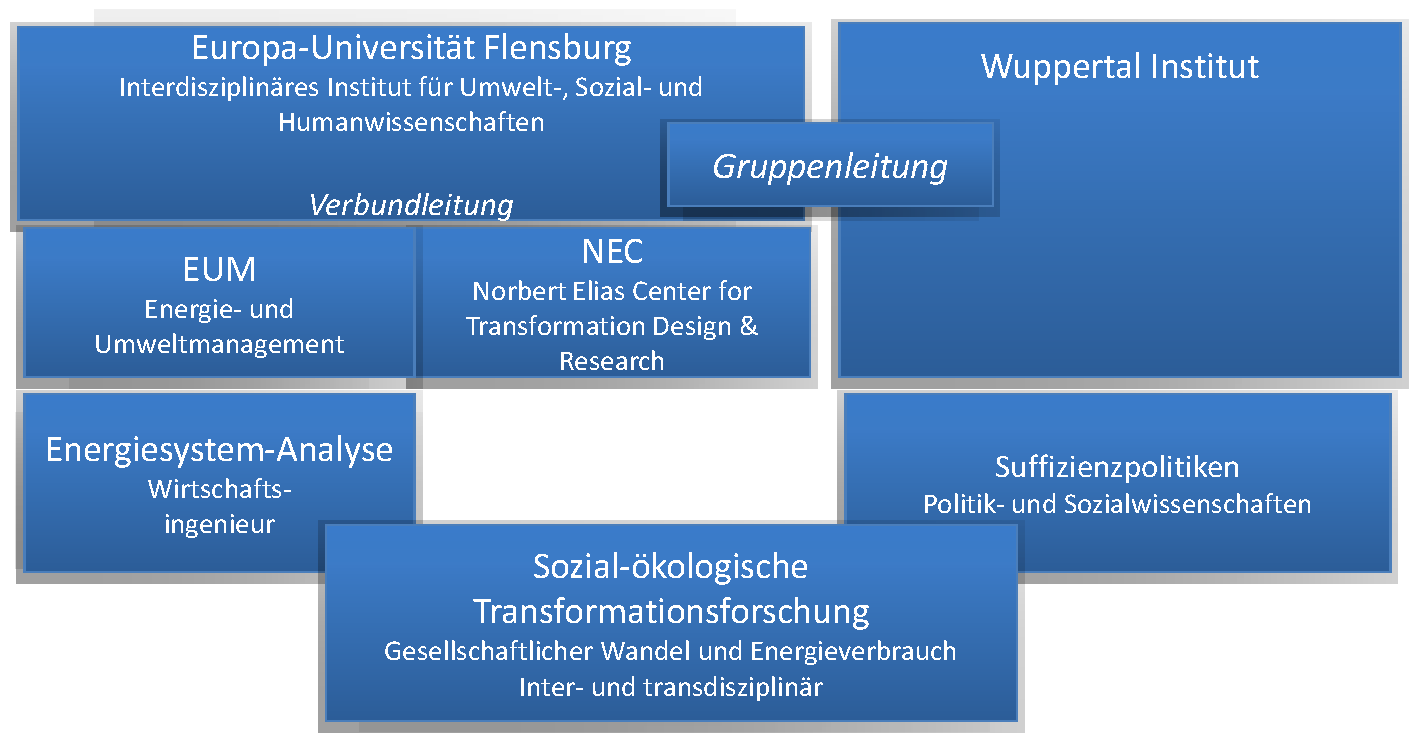
\includegraphics[width=0.8\textwidth]{figures/Konsortium6.pdf}
    \caption{Konsortium}
    \label{fig:konsortium}
\end{figure}

Die Nachwuchsgruppe ist am interdisziplinären Institut für Umwelt-, Sozial- und Humanwissenschaften der EUF und dem WI angesiedelt.
Zur Verstärkung des interdisziplinären Charakters und der engeren Kooperation zwischen Universität und außeruniversitärer Forschungseinrichtung, wird die Forschungsgruppe gemeinsam von Frauke Wiese (EUF) und Benjamin Best (WI) geleitet (siehe CVs im Anhang). Der Forschungsschwerpunkt Energiesystem-Analyse ist in der Abteilung Energie- und Umweltmanagement (EUM) der EUF verortet, während am WI der Forschungsschwerpunkt Suffizienzpolitiken bearbeitet wird. Das NEC (EUF) schlägt mit der sozial-ökologischen Transformationsforschung einen inhaltlichen und interdiziplinären Bogen zwischen Wirtschaftsingenieurwesen sowie Sozial- und Politikwissenschaft.\\ 
Weitere Kooperationen bestehen bereits mit dem Suffizienz-Forschungsnetzwerk, dem Konzeptwerk Neue Ökonomie sowie mit dem inter- und transdisziplinären Netzwerk Vorsorgendes Wirtschaften. Der Bereich Energiesystemanalyse bringt die bereits bestehende Forschungskooperationen mit der Open Energy Modelling Initiative \cite{openmod} ein.
Des Weiteren ist eine enge Zusammenarbeit mit kommunalen Praxispartner*innen bei der Szenarienerstellung und -bewertung geplant. Welche Praxispartner*innen im Nachwuchsforschungsvorhaben in welcher Weise eingebunden werden hängt von der empirischen und theoretischen Schwerpunktsetzung der Qualifikationsarbeiten ab.

\section{Betreuungskonzept}
%\textit{(inklusive der/des vorgesehenen Mentorin bzw. Mentors und Nachweis deren/dessen Expertise in Bezug auf inter- und transdisziplinäre Forschung}

Das Betreuungskonzept sieht vor, die Wachstumsringe der einzelnen Personen und deren Qualifizierungsarbeiten ebenso zu begleiten wie die gemeinsamen Prozesse zu unterstützen. Qualifikationsprozesse bergen zumeist ein Element der „Zwangsisolation“. Daher stellen Nachwuchsprojekte eine vorzügliche Möglichkeit zur Vernetzung und zum Austausch dar; zugleich ist jedoch auf die Möglichkeit für ruhigen Arbeitsphasen zu achten.
Die Gruppenleiterin Frauke Wiese betreut die Promotion in der Energiesystem-Analyse; der Gruppenleiter Benjamin Best die Promotionen im Bereich Suffizienzpolitiken am WI, während die fachliche Betreuung der beiden Promotionen im Bereich sozial-ökologische Transformationsforschung im Rahmen des Transformationskollegs des NECs erfolgt (Leitung: Prof. Dr. Harald Welzer, Koordination und Organisation: Dr. Michaela Christ und Dr. Bernd Sommer) und von jeweils einer der Gruppenleiter*innen interdisziplinär unterstützt wird. Bei der anspruchsvollen Betreuungsaufgabe im Spagat zwischen den Disziplinen unterstützen sich die beiden Nachwuchsgruppenleiter*innen gegenseitig und werden dabei zugleich von der Mentorin unterstützt. Vorgesehen ist Prof. Dr. Uta v. Winterfeld (WI und demnächst auch Universität Kassel), weil sie sowohl disziplinär und formal betreuen als auch inter- und transdisziplinär mitwirken kann (siehe CV im Anhang).\\
Zweimal im Jahr findet ein Reflexionstreffen der Gruppenleiter*innen und der Mentorin statt, mit Fokus auf die Rolle als Leiter*in und den allgemeinen Fortschritt der Forschungsgruppe. Ebenso halbjährlich findet ein Treffen aller Mitarbeiter*innen der Nachwuchsforschungsgruppe einschließlich der Mentorin statt, in der jede*r den Fortschritt des Promotionsprojektes vorstellt. So werden nächste Schritte gemeinsam diskutiert und mögliche Probleme können frühzeitig erkannt und bearbeitet werden.\\
Umwelt- und Transformationsforschung sind per se inter- und transdisziplinär angelegt. Gleichwohl hat sich gezeigt, dass wenig hilfreich ist, wenn alle Beteiligten von ihren Disziplinen absehen und sich naiv gutwillig in einem nicht näher bestimmten inter- und transdisziplinären Raum bewegen. Daher ist das Betreuungskonzept so angelegt, dass einerseits disziplinäre Vergewisserungen erfolgen und andererseits eine Kultur der interdisziplinären Öffnungen gepflegt wird. Hierzu gehört auch, unterstützt durch Weiterbildungsangebote, den disziplinären Blick auf gemeinsame Forschungsgegenstände wie beispielsweise private Haushalte zu werfen. Transdisziplinär wird auf der Betreuungsebene darauf geachtet, dass Praxispartner*innen in den Qualifizierungsarbeiten nicht zu Forschungsobjekten degradiert werden, die ihrerseits im Prozess keine Stimme haben. Vielmehr wird die Subjekt-Objekt-Dialektik kritisch reflektiert. Auch hierzu soll es Weiterbildungsmöglichkeiten geben, die sowohl durch vom Verbund eingeladene Expert*innen als auch durch die Teilnahme an Summer Schools o.Ä. erfolgen kann.\\ 
Die akademische Qualifizierung der Nachwuchswissenschaftler*innen wird sowohl durch Möglichkeiten der Zweitbetreuung von Bachelor- und Masterarbeiten unterstützt als auch dadurch verstärkt, dass von Anfang an eine Kultur des Publizierens gepflegt wird, die in kumulative Promotionen münden können.


\section{Institutionen, Zukunftsperspektiven und Ergebnisverwertung}
%\textit{Darstellung und Motivation der beteiligten Institutionen sowie Zukunftsperspektiven für die jeweiligen Mitglieder der Nachwuchsgruppe (nicht grundfinanzierte außeruniversitäre Forschungsinstitute haben zusätzlich darzustellen, inwieweit den betreffenden Mitgliedern zeitlich befristete Freiräume eingerichtet werden können, sich zeitweise voll auf ihre Qualifikation zu konzentrieren), erwartetes Ergebnis, Anwendungspotenzial und angestrebte Ergebnisverwertung. Der Verwertungsplan muss konkrete Maßnahmen der Öffentlichkeitsarbeit und des Wissenstransfers (auch von Zwischenergebnissen) beinhalten}
An der EUF existiert mit dem Interdisziplinären Institut für Umwelt-, Sozial- und Humanwissenschaften eine zentrale institutionelle Struktur für disziplin-übergreifende Fragestellungen. Die Energie-Suffizienz-Forschungsgruppe soll dort angesiedelt werden. Sie knüpft an die Zusammenarbeit der Abteilung Energie- und Umweltmanagement mit dem sozialwissenschaftlich geprägten NEC an und fügt sich in das Leitbild der EUF ausgezeichnet ein. Die Stärkung der inter- und transdisziplinären Forschung und insbesondere des Themenschwerpunktes Energiewende und Gesellschaft entspricht der Identität und der zukünftigen Entwicklung der Hochschule.\\
Das WI arbeitet interdisziplinär und problemlösungsorientiert im Themenbereich der angewandten Nachhaltigkeitsforschung. Seine Aufgabe ist die Wahrnehmung einer Mittlerfunktion zwischen Wissenschaft, Wirtschaft und Politik. Die Forschungsarbeiten bauen auf disziplinären wissenschaftlichen Erkenntnissen auf und verbinden diese bei der transdisziplinären Bearbeitung komplexer Fragestellungen zu praxisrelevanten und akteursbezogenen Lösungsbeiträgen. Das WI hat den Suffizienzbegriff 1993 in die deutsche Debatte eingebracht (Wolfgang Sachs) und forscht seit einigen Jahren intensiv im Bereich der Suffizienz- und Energie-Suffizienzpolitiken. Es hat Kooperationsbeziehungen vor allem mit den Universtäten Wuppertal und Kassel; eine Intensivierung der Zusammenarbeit mit der EUF ist ebenso naheliegend wie erwünscht.\\
Nach Ablauf des Projektes werden die Nachwuchswissenschaftler*innen mit ihrer inter- und transdisziplinären Erfahrung in einem gesellschaftlich hochaktuellen Thema bestens aufgestellt sein um ihre wissenschaftliche Karriere in diesem Bereich weiterzuführen. An der EUF werden durch eine perspektivische Verstetigung des Forschungsfeldes 'Gesellschaftliche Transformation und Energiewende' Optionen für eine interdisziplinäre akademische Laufbahn in diesem Bereich geschaffen; am WI können außeruniversitäre mit universitären Laufbahnen kombiniert werden. In der letzten Phase der Nachwuchsforschungsgruppe wird der Zukunftsplanung und Analyse der Optionen und Folge-Projekte der beteiligten Wissenschaftler*innen Raum gegeben.\\
Die erarbeiteten Methoden zur konsistenten, integrativen und zur qualitativen Seite hin offenen Szenarienerstellung kann von anderen, speziell interdisziplinär arbeitenden Forscher*innen angewendet und weiterentwickelt werden. Auch das Energiesystem-Modell, dessen Programmier-Code und Daten open source zur Verfügung gestellt werden, bildet eine Basis um auf den Erkenntnissen zu Energie-Suffizienz aufzubauen. Darüber hinaus wird durch die historische Rekonstruktion und die auf die Zukunft gerichteten Szenarien Transformationswissen generiert, das in konkretes Handeln umgesetzt werden kann. Die Forschungsarbeiten am WI werden Erkenntnisse zu Blockaden für und Potenzialen von Energie-Suffizienzpolitiken generieren und damit politische wie zivilgesellschaftliche Transformations- und Innovationsprozesse stärken. Der wissenschaftliche Wissenstransfer wird durch die Teilnahme an Konferenzen und Workshops sowie an Forschungsnetzwerken (Energiewende, Vorsorgendes Wirtschaften, Suffizienz, open energy modelling) sichergestellt. Eine gemeinsame Exkursionsreihe 'Suffizienz-Beispiele in der Praxis' in Zusammenarbeit mit den Praxispartner*innen wird angestrebt.

\section{Zeitplanung und Kostenschätzung}
%\textit{Gesamtkosten bzw. -ausgaben, Grobkalkulation von Personal-, Sach- und Reisemitteln, gegebenenfalls Berücksichtigung von Eigenbeteiligung sowie Drittmitteln).}
Die zeitliche Einordnung und Abfolge der in Abschnitt \ref{sec:4} und beschriebenen Arbeitspakete ist wie folgt vorgesehen:
\begin{figure}[H]
\begin{center}
\resizebox{0.95\textwidth}{!}{
    \begin{ganttchart}[hgrid,
    	vgrid={*{2}{draw=none},dotted},
    	x unit=.65cm,
    	y unit chart=1.75cm,
    	time slot format=isodate-yearmonth,
    	compress calendar,
    	bar/.append style={draw=none,fill=blue},
    	title label font=\Huge\bfseries,
    	group label font=\Huge\bfseries,
    	group/.append style={draw=none,fill=black!50!white},
    	milestone/.append style={draw=none,fill=orange},
    	bar height=.8,
    	group height=.35,
    	milestone height=.75,
    	milestone top shift=.1,
    	milestone label font=\color{orange}
    	]{2019-5}{2024-4}
    	%labels
    	\gantttitle{2019}{8}
    	\gantttitle{2020}{12}
    	\gantttitle{2021}{12}
    	\gantttitle{2022}{12}
    	\gantttitle{2023}{12}
    	\gantttitle{2024}{4} \\
    	\gantttitle{Jahr 1}{12}
    	\gantttitle{Jahr 2}{12}
    	\gantttitle{Jahr 3}{12}
    	\gantttitle{Jahr 4}{12}
    	\gantttitle{Jahr 5}{12}\\
    	%tasks
        \ganttgroup{AP 1}{2019-5}{2020-4}\\
         %   \ganttgroup{}{2020-10}{2021-9}\\
        \ganttgroup{AP 2}{2020-5}{2021-10}\\
        \ganttgroup{AP 3}{2021-1}{2022-4}\\
        \ganttgroup{AP 4}{2021-11}{2023-4}\\
        \ganttgroup{AP 5}{2022-11}{2023-10}\\
        \ganttgroup{AP 6}{2023-4}{2024-4}
    	% \ganttbar[bar/.append style={fill=red}]{AP1.1}{2018-12}{2018-04}\\
    	% \ganttmilestone[inline]{MS1}{2020-6}
    \end{ganttchart}
}
\end{center}
\caption{Gantt-Diagramm der Arbeitspakete}
\label{fig:gantchart}
\end{figure}
Die Kalkulation der Personal-, Reise-, Sach- und Weiterbildungsmittel sind Tabelle \ref{tab:kostenkalkulation} zu entnehmen. Für die gesamten fünf Jahre werden durchgängig vier Stellen beantragt von denen 1,75 Stellen am WI und 2,25 Stellen an der EUF verortet sind. Letztere setzen sich aus einer 0,75-Stelle für die Leitung und drei Doktoranden-Stellen zusammen (halbe Stellen). Am WI wird ebenso eine 0,75-Leitungsstelle (Zusammengesetzt aus 50\% Co-Leitung und 25\% Mentor*innenarbeit, letztere für den gesamten Verbund, sowie zwei halbe Stellen als Doktorandenstellen eingeplant. Zusätzlich werden wissenschaftliche Hilfskräfte für 20 Stunden pro Woche und Forschungsschwerpunkt eingeplant. Es wird ein Overhead von 20\% für die EUF und von 90\% für die außeruniversitäre Forschungseinrichtung WI veranschlagt. Der Eigenanteil des WI beträgt 10\%.\\
In den Reisemitteln sind die Teilnahme an Konferenzen ab dem zweiten Jahr sowie an den Workshops pro Person und Jahr enthalten. Außerdem wurde mit halbjährlichen Treffen abwechselnd in Wuppertal und in Flensburg mit allen Personen und zusätzlichen bilateralen Treffen pro Jahr kalkuliert. In den Sachmitteln sind neben Literatur und Computer für die Modellierung ab dem zweiten Jahr Gelder für Open Access Veröffentlichungen enthalten. In die Kategorie Weiterbildung fallen Kursgebühren für Qualifizierungsworkshops und Summer Schools.

\begin{table}[h]
\begin{center}
  \caption{Abschätzung der Gesamtkosten je Kostenkategorie für Energie- und Umweltmanagement (EUM) und Norbert Elias Center (NEC) (beide EUF) und Wuppertal Institut}
\small  
\begin{tabular}[h]{|l | r | r | r | r|}
\hline
&&&&\\
& EUF EUM & EUF NEC & Wuppertal Institut & \textbf{Summe in Euro}\\
\hline
\hline
&&&&\\
 Personalmittel & 630.440 & 495.520 & 1.474.710 & 2.600.670\\
 \hline
 &&&&\\
 Reisemittel & 54.000 & 54.000 & 50.000 & 158.000\\
 \hline
 &&&&\\
 Sachmittel & 28.200 & 28.200 & 30.000 & 86.400\\
 \hline
 &&&&\\
 Weiterbildung & 15.600 & 15.600 & 15.000 & 46.200\\
 \hline
 \hline
 &&&&\\
 \textbf{Summe}& \textbf{728.240} & \textbf{593.320} & \textbf{1.569.710} & \underline{\textbf{2.891.270}}\\
 \hline
 \end{tabular}
 \label{tab:kostenkalkulation}
\end{center}
\end{table}

Tabelle \ref{tab:kostenkalkulation2} fasst die Kosten je Institution sowie die beantragte Zuwendung entsprechend der Förderquote zusammen.

\begin{table}[h]
\small
\begin{center}
  \caption{Abschätzung von Gesamtkosten und beantragter Förderung je Institution}
\begin{tabular}[h]{|l | r | r | r|}
\hline
&&&\\
Institution & Kosten [Euro] & Förderquote [\%] & \textbf{beantragte Zuwendung}\\
\hline
\hline
 &&&\\
 EUF & 1.321.560 & 100 & 1.321.560\\
 \hline
 &&&\\
 Wuppertal Institut & 1.569.710 & 90 & 1.412.739
\\
 \hline
 \hline
 &&&\\
 \textbf{Gesamt} & & &\underline{\textbf{2.734.299}}\\
 \hline
 \end{tabular}
 \label{tab:kostenkalkulation2}
\end{center}
\end{table}

\clearpage
\footnotesize
%\sectionp*{Literatur} \label{sec:lit}
%\bibliographystyle{plainnat}%elsarticle-num}
%\bibliographystyle{abbrvdin}
%\bibliographystyle{natdin}
%\bibliographystyle{plaindin}
\bibliographystyle{unsrtdin}
%\bibliographystyle{unsrtnat}
%\bibliographystyle{elsarticle-num}
%\bibliographystyle{apalike}
%\bibliographystyle{alphadin}
%\bibliographystyle{abbrvnat}
\bibliography{literature.bib}

%\clearpage
%\appendix

%\section{Anhang}

%\textit{Literaturlisten, Lebensläufe und gegebenenfalls Interessensbekundungen von Praxispartnern sind im Anhang beizufügen.}

%\section{Projekte}
%Für die Übersicht sind die Projekte hier nochmal aufgeführt

%\section{Lebensläufe}

\end{document}
